\documentclass{article}%
\usepackage[T1]{fontenc}%
\usepackage[utf8]{inputenc}%
\usepackage{lmodern}%
\usepackage{textcomp}%
\usepackage{lastpage}%
%
\usepackage{amsmath}%
\usepackage{amssymb}%
\usepackage{amsfonts}%
\usepackage{graphicx}%
\usepackage{hyperref}%
\usepackage{tikz}%
\usepackage{pgfplots}%
\usetikzlibrary{math}%
\title{ITA 2027 - Física (one-shot, sem judge)\thanks{This exam was solved and automatically generated with gpt-resolve: \url{https://github.com/lgabs/gpt-resolve}}}%
\author{claude{-}opus{-}5{-}5}%
\date{October 30, 2026}%
%
\begin{document}%
\normalsize%
\maketitle%
\section*{Questão 1}

\section*{Solução}

\textbf{Modelo.} Tomamos $\theta$ positivo no sentido da figura. Sobre a haste (corpo rígido que gira em torno do eixo fixo no polímero) atuam o torque elástico $\tau_e=-k\theta$ e o torque do peso, aplicado no centro de massa (ponto médio, a $L/2$ do eixo):
\[
\tau_P=+Mg\,\frac{L}{2}\,\operatorname{sen}\theta ,
\]
que tende a \emph{aumentar} $|\theta|$ (pêndulo invertido). Ambos os torques são conservativos, com
\[
U_{total}(\theta)=\underbrace{\tfrac12 k\theta^2}_{\text{elástica}}+\underbrace{Mg\,\tfrac{L}{2}\cos\theta}_{\text{gravitacional (zero no mancal)}},
\qquad
\tau=-\frac{dU_{total}}{d\theta}=-k\theta+\frac{MgL}{2}\operatorname{sen}\theta .
\]

\textbf{a)} Para $|\theta|\ll 1$, $\operatorname{sen}\theta\approx\theta$ e
$\tau\approx-\left(k-\tfrac{MgL}{2}\right)\theta$. O torque é restaurador (equilíbrio estável, com oscilações de $\omega^2=\frac{k-MgL/2}{ML^2/3}>0$) somente se $k>MgL/2$; se $k<MgL/2$, o torque afasta a haste da vertical. Logo
\[
\boxed{k_c=\frac{MgL}{2}}\qquad(\text{unidade: N}\cdot\text{m/rad, coerente com }k).
\]
No caso limite $k=k_c$: $U_{total}-U_{total}(0)=k_c\left(\tfrac{\theta^2}{2}+\cos\theta-1\right)\approx k_c\,\tfrac{\theta^4}{24}>0$, de modo que $\theta=0$ ainda é estável (mínimo quártico), em acordo com o enunciado (é $k<k_c$ que desestabiliza).

\textbf{b)} Com $k_c=MgL/2$ e $r\equiv k/k_c>0$, os equilíbrios ($\tau=0$) satisfazem
\[
k\theta=k_c\operatorname{sen}\theta\iff \theta=0\quad\text{ou}\quad \frac{\operatorname{sen}\theta}{\theta}=r .
\]
Em $0<|\theta|<\pi/2$ a função par $f(\theta)=\operatorname{sen}\theta/\theta$ decresce estritamente de $1$ (em $\theta\to0$) até $2/\pi$ (em $|\theta|=\pi/2$). Além disso, $U_{total}''(\theta)=k-k_c\cos\theta$, logo $U_{total}''(0)=k_c(r-1)$. Daí:

\begin{itemize}
\item \textbf{$r\ge1$:} $f(\theta)<1\le r$ para $\theta\neq0$ $\Rightarrow$ \textbf{um único} equilíbrio, $\theta=0$, \textbf{estável} ($U_{total}''(0)>0$; para $r=1$, mínimo quártico do item a).
\item \textbf{$2/\pi<r<1$:} \textbf{três} equilíbrios. $\theta=0$ é \textbf{instável} ($U_{total}''(0)<0$); $\theta=\pm\theta_e$, com $\dfrac{\operatorname{sen}\theta_e}{\theta_e}=\dfrac{k}{k_c}$ ($0<\theta_e<\pi/2$), são \textbf{estáveis}: para $\theta>\theta_e$ tem-se $f(\theta)<r$, isto é, $k\theta>k_c\operatorname{sen}\theta$ e $\tau<0$; para $0<\theta<\theta_e$, $\tau>0$; o torque sempre empurra a haste de volta para $\theta_e$ (idem para $-\theta_e$, por simetria). Equivalentemente, $U_{total}''(\theta_e)=k_c\cos\theta_e\,\frac{\tan\theta_e-\theta_e}{\theta_e}>0$.
\item \textbf{$0<r\le2/\pi$:} $f(\theta)>2/\pi\ge r$ em todo o intervalo aberto $\Rightarrow$ \textbf{um único} equilíbrio, $\theta=0$, \textbf{instável}; o torque afasta a haste da vertical até ela sair do intervalo (tomba até $|\theta|=\pi/2$, sobre o suporte). Em $r=2/\pi$ ($k=MgL/\pi$) os pontos $\pm\theta_e$ chegam exatamente a $\pm\pi/2$, fora do intervalo aberto.
\end{itemize}
Interpretação do ensaio: ao aquecer, a haste fica vertical até $k=k_c$; depois inclina-se para um dos lados ($\pm\theta_e$, quebra de simetria), com $\theta_e$ crescendo continuamente ($\theta_e\approx\sqrt{6(1-r)}$ para $r\to1^-$), e tomba quando $k\to MgL/\pi$.

\textbf{c)} $\dfrac{U_{total}}{k_c}=\dfrac{r}{2}\theta^2+\cos\theta$, função par, com $U_{total}(0)=\dfrac{MgL}{2}$ (centro de massa a $L/2$ acima do mancal) e $U_{total}(\pm\pi/2)=\dfrac{\pi^2k}{8}$ (haste horizontal: energia gravitacional nula). Esboços (curvas exatas para $r=1{,}5$ e $r=1$; $r=0{,}75$; $r=0{,}4$):

\begin{center}
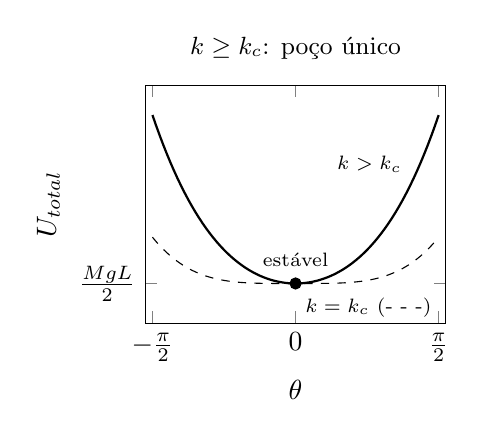
\begin{tikzpicture}
\begin{axis}[width=5.4cm,height=4.6cm,domain=-pi/2:pi/2,samples=81,
  xmin=-1.65,xmax=1.65,xtick={-1.5708,0,1.5708},xticklabels={$-\frac{\pi}{2}$,$0$,$\frac{\pi}{2}$},
  ytick={1},yticklabels={$\frac{MgL}{2}$},ymin=0.8,ymax=2.0,
  title={\small $k\ge k_c$: poço único},xlabel={$\theta$},ylabel={$U_{total}$}]
\addplot[thick] {0.75*x^2+cos(deg(x))};
\addplot[dashed] {0.5*x^2+cos(deg(x))};
\addplot[only marks,mark=*] coordinates {(0,1)};
\node[font=\scriptsize] at (axis cs:0,1.12) {estável};
\node[font=\scriptsize,anchor=west] at (axis cs:0.35,1.6) {$k>k_c$};
\node[font=\scriptsize] at (axis cs:0.8,0.88) {$k=k_c$ (- - -)};
\end{axis}
\end{tikzpicture}\hfill
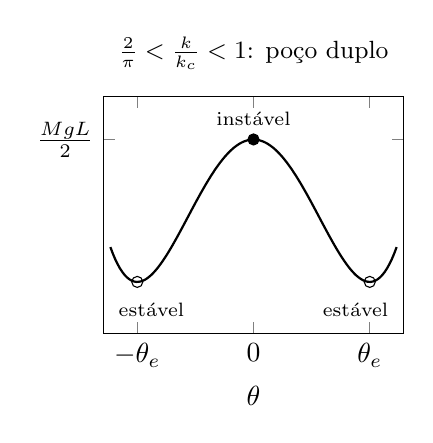
\begin{tikzpicture}
\begin{axis}[width=5.4cm,height=4.6cm,domain=-pi/2:pi/2,samples=121,
  xmin=-1.65,xmax=1.65,xtick={-1.2757,0,1.2757},xticklabels={$-\theta_e$,$0$,$\theta_e$},
  ytick={1},yticklabels={$\frac{MgL}{2}$},ymin=0.865,ymax=1.03,
  title={\small $\frac{2}{\pi}<\frac{k}{k_c}<1$: poço duplo},xlabel={$\theta$}]
\addplot[thick] {0.375*x^2+cos(deg(x))};
\addplot[only marks,mark=*] coordinates {(0,1)};
\addplot[only marks,mark=o] coordinates {(-1.2757,0.9011) (1.2757,0.9011)};
\node[font=\scriptsize,anchor=south] at (axis cs:0,1.003) {instável};
\node[font=\scriptsize,anchor=north] at (axis cs:-1.12,0.893) {estável};
\node[font=\scriptsize,anchor=north] at (axis cs:1.12,0.893) {estável};
\end{axis}
\end{tikzpicture}\hfill
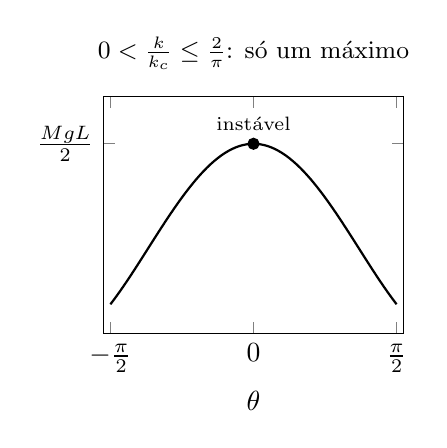
\begin{tikzpicture}
\begin{axis}[width=5.4cm,height=4.6cm,domain=-pi/2:pi/2,samples=81,
  xmin=-1.65,xmax=1.65,xtick={-1.5708,0,1.5708},xticklabels={$-\frac{\pi}{2}$,$0$,$\frac{\pi}{2}$},
  ytick={1},yticklabels={$\frac{MgL}{2}$},ymin=0.4,ymax=1.15,
  title={\small $0<\frac{k}{k_c}\le\frac{2}{\pi}$: só um máximo},xlabel={$\theta$}]
\addplot[thick] {0.2*x^2+cos(deg(x))};
\addplot[only marks,mark=*] coordinates {(0,1)};
\node[font=\scriptsize,anchor=south] at (axis cs:0,1.01) {instável};
\end{axis}
\end{tikzpicture}
\end{center}

\begin{itemize}
\item $k\ge k_c$: curva em ``U'' (convexa, pois $U_{total}''=k-k_c\cos\theta\ge0$), mínimo $MgL/2$ em $\theta=0$; para $k=k_c$ o fundo é achatado ($\propto\theta^4$).
\item $2/\pi<k/k_c<1$: curva em ``W'': máximo local $MgL/2$ em $\theta=0$ e dois mínimos simétricos em $\pm\theta_e$ (abaixo de $MgL/2$).
\item $0<k/k_c\le2/\pi$: curva em ``$\cap$'': máximo em $\theta=0$ e $U_{total}$ decrescendo monotonamente até $\pi^2k/8\le\frac{\pi}{4}\cdot\frac{MgL}{2}$ nas extremidades.
\end{itemize}

ANSWER: a) $k_c=\dfrac{MgL}{2}$. b) Para $k/k_c\ge1$: um equilíbrio, $\theta=0$, estável. Para $2/\pi<k/k_c<1$: três equilíbrios, $\theta=0$ instável e $\theta=\pm\theta_e$ estáveis, com $\operatorname{sen}\theta_e/\theta_e=k/k_c$. Para $0<k/k_c\le2/\pi$: um equilíbrio, $\theta=0$, instável. c) $U_{total}=\tfrac12k\theta^2+\tfrac{MgL}{2}\cos\theta$: poço único (``U'') com mínimo $MgL/2$ em $0$; poço duplo (``W'') com máximo $MgL/2$ em $0$ e mínimos em $\pm\theta_e$; curva em ``$\cap$'' com máximo em $0$, decrescendo até $\pi^2k/8$ em $\pm\pi/2$.
%
\newpage%
\section*{Questão 2}

\section*{Solução}

\textbf{Hipóteses.} O solo é horizontal e liso, a resistência do ar é desprezada e o choque é instantâneo. Tomamos o eixo $x$ na horizontal, o eixo $y$ na vertical para cima e a energia potencial nula no solo.

\textbf{Componentes da velocidade.} No lançamento,
\[
v_x = V\cos 30^\circ = \frac{\sqrt{3}}{2}V, \qquad v_{y,0} = V\,\mathrm{sen}\, 30^\circ = \frac{V}{2}.
\]
\begin{itemize}
\item \emph{Entre os choques:} a única força é o peso, que é vertical. Logo $v_x$ é constante, o movimento vertical é um MUV e a energia mecânica se conserva.
\item \emph{No choque:} como o solo é liso, não há atrito e o impulso do solo é só normal (vertical). Assim, $v_x$ não muda. Na vertical, pela definição do coeficiente de restituição (o solo fica parado),
\[
e=\frac{|v_y'|}{|v_y|}\;\Rightarrow\; v_{y,k}=e\,v_{y,k-1}\;\Rightarrow\; v_{y,n}=e^{n}\,\frac{V}{2}.
\]
Aqui $v_{y,n}$ é a componente vertical logo após o $n$-ésimo choque. Pela simetria do MUV, o corpo chega ao solo com a mesma componente vertical, em módulo, com que saiu dele.
\end{itemize}

\textbf{a) Altura máxima após $n$ choques.} No ponto mais alto, $v_y=0$. Por Torricelli na vertical,
\[
H_n=\frac{v_{y,n}^2}{2g}=\frac{e^{2n}}{2g}\cdot\frac{V^2}{4}=\frac{(0{,}49)^n\,V^2}{8g}.
\]
\emph{Verificação:} para $n=0$ obtemos $V^2/(8g)$, que é a altura máxima do lançamento oblíquo usual. A cada choque a altura fica multiplicada por $e^2=0{,}49$.

\textbf{b) Tempo até a energia mínima.} Logo após o $k$-ésimo choque (no solo, $U=0$), a energia mecânica é
\[
E_k=\frac{1}{2}m v_x^2+\frac{1}{2}m v_{y,k}^2=\frac{3mV^2}{8}+\frac{mV^2}{8}(0{,}49)^k .
\]
\begin{itemize}
\item A energia só diminui nos choques, e cada choque dissipa a fração $1-e^2=0{,}51$ da energia cinética vertical.
\item A parcela horizontal $\tfrac{1}{2}mv_x^2$ não pode ser dissipada, porque nenhuma força horizontal atua sobre o corpo.
\end{itemize}
Portanto, a energia mínima é
\[
E_{\min}=\frac{3mV^2}{8},
\]
atingida quando $v_y\to 0$. Isso exige infinitos choques, mas em tempo finito.

\emph{Cálculo do tempo.} O voo que começa com componente vertical $v_{y,k}$ dura
\[
t_k=\frac{2v_{y,k}}{g}=\frac{V}{g}\,e^{k}.
\]
Somando a série geométrica de razão $e=0{,}7<1$ (convergente):
\[
\Delta t=\sum_{k=0}^{\infty}\frac{V}{g}\,e^{k}=\frac{V}{g}\cdot\frac{1}{1-e}=\frac{V}{0{,}3\,g}=\frac{10V}{3g}.
\]
Nesse instante, $y\to 0$ e $v_y\to 0$. A partir dele, a massa desliza sobre o solo liso com velocidade constante $\frac{\sqrt{3}}{2}V$ e a energia permanece no mínimo. Nesse intervalo, a massa percorre a distância horizontal $x=v_x\,\Delta t=\dfrac{5\sqrt{3}\,V^2}{3g}$.

\emph{Conferências:}
\begin{itemize}
\item Unidades: $[V/g]=\mathrm{s}$ e $[V^2/g]=\mathrm{m}$.
\item Ordem de grandeza: para $V=10$ m/s, $\Delta t\approx 3{,}4$ s, cerca de $3{,}3$ vezes a duração do primeiro voo ($V/g$).
\end{itemize}

ANSWER: a) $H_n=\dfrac{(0{,}49)^n V^2}{8g}$; b) $\Delta t=\dfrac{V}{g(1-e)}=\dfrac{10V}{3g}$, quando a energia atinge o mínimo $E_{\min}=\dfrac{3mV^2}{8}$ (só resta a energia cinética horizontal).%
\newpage%
\section*{Questão 3}

\section*{Solução}

\textbf{Hipóteses.} A massa é tratada como ponto e o ar não oferece resistência. A origem $O$ fica no solo, sobre o eixo de rotação, e a borda do carrossel está a uma distância $R$ desse eixo. Como a massa está na borda, ela deixa o disco no mesmo instante em que perde a aderência, com a velocidade que tinha nesse momento. Supõe-se $\mu_e g > \alpha R$; caso contrário, ela escorregaria já em $t=0$, ainda sem velocidade.

\textbf{1) Início do escorregamento.} Enquanto não escorrega, a massa descreve um MCUV de raio $R$, com $\omega(t)=\alpha t$. Sua aceleração horizontal tem duas componentes:
\[
a_t=\alpha R \quad (\text{tangencial}), \qquad a_c=\omega^2R=\alpha^2t^2R \quad (\text{centrípeta}).
\]
O peso e a normal são verticais, e por isso $N=mg$. A única força horizontal é o atrito estático. Pela 2.ª lei de Newton,
\[
f=m\sqrt{a_t^2+a_c^2}=mR\alpha\sqrt{1+\alpha^2t^4},
\]
que cresce com $t$. O escorregamento começa quando $f$ atinge o valor máximo $\mu_e N=\mu_e mg$:
\[
R\alpha\sqrt{1+\alpha^2t_1^4}=\mu_e g \;\Longrightarrow\; t_1=\frac{\left[(\mu_e g)^2-(\alpha R)^2\right]^{1/4}}{\alpha\sqrt{R}} .
\]
Nesse instante, $\omega_1=\alpha t_1$, e a velocidade da massa é tangente à borda:
\[
v_0=\omega_1R=\sqrt{R}\,\left[(\mu_e g)^2-(\alpha R)^2\right]^{1/4}
\quad\Longrightarrow\quad v_0^2=R\sqrt{\mu_e^2g^2-\alpha^2R^2}.
\]
No referencial do disco, a resultante das forças de inércia não equilibradas tem uma componente radial para fora, igual a $m\omega_1^2R>0$. Por isso a massa desliza para fora e abandona o carrossel. Pela continuidade da velocidade, ela sai com $\vec v_0$ horizontal e tangente à borda.

\textbf{a)} A partir daí, a massa é um projétil lançado horizontalmente de altura $h$. O tempo de queda é $t_q=\sqrt{2h/g}$. Na horizontal o movimento é uniforme, e o deslocamento é $d=v_0t_q$, ao longo da tangente. Seja $P'$ a projeção no solo do ponto de saída; então $OP'=R$. Como a tangente é perpendicular ao raio, $OP'\perp P'Q$, onde $Q$ é o ponto de contato com o solo. Pelo teorema de Pitágoras,
\[
D=OQ=\sqrt{R^2+v_0^2\,\frac{2h}{g}}=\sqrt{R^2+\frac{2hR}{g}\sqrt{\mu_e^2g^2-\alpha^2R^2}} .
\]
O resultado não depende do ângulo $\theta_1=\alpha t_1^2/2$ girado até a saída.

\textbf{b)} Ao tocar o solo, a massa não quica: o choque anula a componente vertical da velocidade e mantém a horizontal $v_0$. O choque é considerado instantâneo. Durante o deslizamento, $N=mg$, e o atrito cinético $\mu_c mg$ se opõe à velocidade. O movimento é então retilíneo e uniformemente retardado, com desaceleração $\mu_c g$, e a massa para após $t_d=v_0/(\mu_c g)$. O instante da parada é
\[
t_p=t_1+t_q+t_d=\frac{\left[(\mu_e g)^2-(\alpha R)^2\right]^{1/4}}{\alpha\sqrt{R}}+\sqrt{\frac{2h}{g}}+\frac{\sqrt{R}\,\left[(\mu_e g)^2-(\alpha R)^2\right]^{1/4}}{\mu_c g}.
\]

\textbf{Verificações.}
\begin{itemize}
\item \emph{Unidades:} $[(\mu_e g)^2]^{1/4}=(\mathrm{m/s^2})^{1/2}$. Assim, $t_1$ resulta em s, $v_0$ em m/s e $D$ em m.
\item \emph{Limite $\alpha\to 0$:} obtém-se $v_0^2\to\mu_e gR$, que é a velocidade máxima clássica numa curva com atrito. Nesse limite, $D\to\sqrt{R^2+2\mu_e hR}$ e $t_1\to\infty$, pois o disco leva um tempo arbitrariamente longo para ganhar velocidade.
\item \emph{Limite $\alpha R\to\mu_e g$:} obtém-se $t_1\to0$, $v_0\to0$, $D\to R$ (queda vertical) e $t_p\to\sqrt{2h/g}$.
\item \emph{Ordem de grandeza:} com $R=2$ m, $\alpha=0{,}5$ rad/s$^2$, $\mu_e=0{,}4$, $\mu_c=0{,}3$ e $h=1{,}2$ m, obtêm-se $t_1\approx2{,}75$ s, $D\approx2{,}42$ m e $t_p\approx4{,}18$ s. São valores plausíveis.
\end{itemize}

\textbf{Observação.} Esta é uma hipótese alternativa. Se também se considerasse o atrito impulsivo durante o choque, de impulso $\mu_c\,m\sqrt{2gh}$, a velocidade horizontal após o choque seria $v_0-\mu_c\sqrt{2gh}$, e o termo $\sqrt{2h/g}$ se cancelaria. O resultado seria $t_p=t_1+v_0/(\mu_c g)$, válido se $v_0\ge\mu_c\sqrt{2gh}$. Adotou-se aqui a interpretação usual do enunciado.

ANSWER: a) $D=\sqrt{R^2+\dfrac{2hR}{g}\sqrt{\mu_e^2g^2-\alpha^2R^2}}$; \quad b) $t_p=\dfrac{\left[(\mu_e g)^2-(\alpha R)^2\right]^{1/4}}{\alpha\sqrt{R}}+\sqrt{\dfrac{2h}{g}}+\dfrac{\sqrt{R}\left[(\mu_e g)^2-(\alpha R)^2\right]^{1/4}}{\mu_c g}$%
\newpage%
\section*{Questão 4}

\section*{Solução}

\textbf{Hipóteses.} Gás ideal monoatômico: $U=\tfrac32 nRT=\tfrac32 PV$ e $\gamma=C_P/C_V=\tfrac53$. Paredes e pistão são adiabáticos, então $Q=0$. Há vácuo acima do pistão, logo a única força externa sobre ele, além da do gás, é o peso. O volume do gás é $V=Ah$.

\textbf{Estado inicial.} O pistão sustenta a areia, então no equilíbrio
\[
P_iA=(m+M)g \;\Rightarrow\; P_iV_i=(m+M)g\,h_i .
\]

\subsection*{a) Retirada lenta (quase estática)}
Em cada instante o pistão está em equilíbrio e o gás passa por estados de equilíbrio. Sem troca de calor, o processo é uma adiabática reversível:
\[
PV^{\gamma}=\text{cte},\qquad P_f=\frac{mg}{A}\ \ (\text{sem areia}).
\]
Então
\[
\frac{(m+M)g}{A}\,(Ah_i)^{5/3}=\frac{mg}{A}\,(Ah_f)^{5/3}
\;\Rightarrow\;
\boxed{h_f=h_i\left(\frac{m+M}{m}\right)^{3/5}}
\]
Verificações: o resultado é adimensional na razão $h_f/h_i$. Para $M\to 0$ tem-se $h_f\to h_i$, e $h_f>h_i$ sempre, como esperado numa expansão.

\subsection*{b) Retirada instantânea}
Logo após a retirada, o pistão ainda está em repouso em $h_i$. A força resultante $P_iA-mg=Mg$ aponta para cima, então o pistão acelera para cima, passa da posição de equilíbrio e para momentaneamente em $h_{max}$, que é um ponto de retorno de uma oscilação. Como a areia sai instantaneamente e com velocidade nula, ela não realiza trabalho sobre o pistão.

\textbf{Gás.} Não há atrito e a massa do gás é desprezível. Supomos também que o pistão se move devagar em comparação com a velocidade do som no gás. Assim, o gás permanece uniforme e evolui por uma adiabática reversível:
\[
PV=P_iV_i\left(\frac{V_i}{V}\right)^{\gamma-1}
\;\Rightarrow\;
P_{max}V_{max}=(m+M)g\,h_i\left(\frac{h_i}{h_{max}}\right)^{2/3}.
\]
Pela 1ª lei com $Q=0$, o trabalho do gás é
\[
W_{gás}=-\Delta U=\tfrac32\left(P_iV_i-P_{max}V_{max}\right).
\]

\textbf{Pistão (teorema da energia cinética).} Entre $h_i$ e $h_{max}$ o pistão parte do repouso e chega ao repouso, então $\Delta K=0$:
\[
W_{gás}-mg\,(h_{max}-h_i)=0 .
\]
Substituindo e cancelando $g$:
\[
\boxed{\;\frac32\,(m+M)\,h_i\left[1-\left(\frac{h_i}{h_{max}}\right)^{2/3}\right]=m\,(h_{max}-h_i)\;}
\]
Em forma equivalente:
\[
3(m+M)h_i\left[1-\left(\frac{h_i}{h_{max}}\right)^{2/3}\right]=2m\,(h_{max}-h_i).
\]

\textbf{Discussão da raiz.} Sejam $x=h/h_i$ e $k=(m+M)/m$. Defina
\[
f(x)=\tfrac32k\,(1-x^{-2/3})-(x-1),
\]
que é proporcional à energia cinética do pistão na altura $x$. Temos:
\begin{itemize}
\item $f(1)=0$, que é o ponto de partida;
\item $f'(x)=kx^{-5/3}-1$, que se anula em $x=k^{3/5}=h_f/h_i$, isto é, a energia cinética é máxima na posição de equilíbrio do item a);
\item $f''(x)<0$.
\end{itemize}
Logo existe uma única outra raiz, e ela é maior que $h_f/h_i$, ou seja, $h_{max}>h_f$.

\textbf{Casos particulares.}
\begin{itemize}
\item $M\to 0$: $h_{max}\to h_i$, pois não há movimento.
\item $M\ll m$: as oscilações são pequenas, quase harmônicas, e $h_{max}\approx 2h_f-h_i$.
\item Exemplo com $M=m$: $h_f\approx 1{,}52\,h_i$ e $h_{max}\approx 2{,}26\,h_i$.
\end{itemize}

ANSWER: a) $h_f=h_i\left(\dfrac{m+M}{m}\right)^{3/5}$; b) $\dfrac32(m+M)h_i\left[1-\left(\dfrac{h_i}{h_{max}}\right)^{2/3}\right]=m\,(h_{max}-h_i)$%
\newpage%
\section*{Questão 5}

\section*{Solução}

\textbf{Convenções.} Eixo $x$ sobre o eixo de simetria, origem no vértice $V$, luz indo do meio $n_1$ (esquerda) para o meio $n_2$ (direita). O centro de curvatura $C$ está no meio $n_1$, em $x=-R$; as fontes estão em $x=-p$, $y=\pm h$. Aproximação paraxial: ângulos pequenos, $\operatorname{sen}\theta\approx\tan\theta\approx\theta$.

\textbf{a) Posição horizontal.} Um raio que sai do ponto axial $O$ ($x=-p$) atinge o dioptro em $I$, a uma altura $y$. Em relação ao eixo, o raio incidente faz o ângulo $\alpha\approx y/p$ e a normal $CI$ faz $\varphi\approx y/R$. O ângulo de incidência é então $\theta_1=\alpha-\varphi$, e a lei de Snell paraxial dá $n_1\theta_1=n_2\theta_2$. O raio refratado faz com o eixo o ângulo
\[
\beta=\varphi+\theta_2=\frac{y}{R}+\frac{n_1}{n_2}\left(\frac{y}{p}-\frac{y}{R}\right)=\frac{y}{n_2}\left[\frac{n_1}{p}+\frac{n_2-n_1}{R}\right]>0 .
\]
Como $\beta>0$, o raio refratado se afasta do eixo e só o seu prolongamento corta o eixo, à esquerda de $V$, na distância $y/\beta$ (independe de $y$, então há imagem):
\[
|p'|=\frac{n_2\,p\,R}{n_1R+(n_2-n_1)\,p}
\qquad\Big(\text{com sinal: } p'=-\frac{n_2pR}{n_1R+(n_2-n_1)p}\Big).
\]
Isso é a equação do dioptro $\dfrac{n_1}{p}+\dfrac{n_2}{p'}=\dfrac{n_2-n_1}{R_{\text{alg}}}$ com $R_{\text{alg}}=-R$ (centro do lado da luz incidente). Como $n_2>n_1$, a imagem é \emph{virtual}: fica no meio $n_1$, a uma distância $|p'|$ à esquerda do vértice.

\textbf{Posições verticais.} O raio que sai da fonte $(-p,\,h)$ passando por $C$ incide na direção da normal e não sofre desvio. Logo, a imagem fica sobre a reta $C F$ e na abscissa $x=-|p'|$:
\[
y'=h\,\frac{R-|p'|}{R-p},\qquad R-|p'|=\frac{n_1R\,(R-p)}{n_1R+(n_2-n_1)p}
\;\Longrightarrow\;
y'=\pm\,\frac{n_1R}{n_1R+(n_2-n_1)\,p}\,h .
\]
As imagens são direitas e reduzidas, com aumento $m=\dfrac{n_1R}{n_1R+(n_2-n_1)p}<1$, e ficam separadas por $2|y'|$. \emph{Verificações:} para $R\to\infty$ (dioptro plano), $|p'|=\dfrac{n_2}{n_1}p$ e $y'=\pm h$, que é a profundidade aparente usual. Para $p=R$ (objeto em $C$), a imagem também fica em $C$ e $m=n_1/n_2$, que é o resultado clássico. Uma traçagem exata de raios ($n_1=1$, $n_2=1{,}5$, $R=0{,}3$ m, $p=0{,}1$ m) confirma $|p'|=0{,}1286$ m.

\textbf{b) Caso $R\to\infty$.} Pelo item (a), no meio $n_2$ a luz parece vir de duas fontes virtuais $F_1'$ e $F_2'$, situadas em $x=-\dfrac{n_2p}{n_1}$, $y=\pm h$. Elas estão separadas por $d=2h$ e ficam à distância $L=D+\dfrac{n_2p}{n_1}$ da tela. Pela simetria em relação ao eixo, os caminhos ópticos de cada fonte real até sua frente de onda virtual são iguais, então $F_1'$ e $F_2'$ são coerentes e estão em fase. Temos portanto um experimento de Young imerso no meio $n_2$, onde o comprimento de onda vale $\lambda/n_2$ ($\lambda$ é o comprimento de onda no vácuo).

Num ponto da tela de altura $y$, com $h,\,y\ll L$, a diferença de caminho óptico é
\[
\Delta = n_2\big(\overline{F_2'P}-\overline{F_1'P}\big)\approx n_2\,\frac{2h\,y}{L}.
\]
Há máximo quando $\Delta=k\lambda$. Para $k=0$ temos $y=0$: é o ponto luminoso central. Para $k=1$:
\[
y_1=\frac{\lambda L}{2n_2h}=\frac{\lambda}{2n_2h}\left(D+\frac{n_2}{n_1}p\right)\approx\frac{\lambda D}{2\,n_2\,h}\quad (p\ll D).
\]
\emph{Conferência direta por Snell:} raios paralelos que saem das fontes com ângulo $\theta_1$ no meio $n_1$ têm diferença de caminho óptico $n_1(2h)\theta_1=n_2(2h)\theta_2$. Eles chegam à tela em $y\approx p\theta_1+D\theta_2=\theta_2\left(D+\tfrac{n_2}{n_1}p\right)$, o que leva ao mesmo resultado.

A unidade de $\lambda D/h$ é de comprimento. Para $\lambda=600$ nm, $D=1$ m, $h=0{,}5$ mm e $n_2=1{,}5$, obtemos $y_1\approx0{,}4$ mm, um valor razoável. Para $n_2=1$, recupera-se o Young usual, $\lambda D/d$. (Se $\lambda$ fosse o comprimento de onda no meio $n_1$, bastaria trocar $\lambda$ por $n_1\lambda$, o que dá $n_1\lambda D/(2n_2h)$.)

\medskip
\noindent ANSWER: a) $p'=-\dfrac{n_2pR}{n_1R+(n_2-n_1)p}$ (imagem virtual, a $\dfrac{n_2pR}{n_1R+(n_2-n_1)p}$ à esquerda do vértice, no meio $n_1$); alturas $y'=\pm\dfrac{n_1R}{n_1R+(n_2-n_1)p}\,h$. b) $\Delta y=\dfrac{\lambda}{2n_2h}\left(D+\dfrac{n_2p}{n_1}\right)\approx\dfrac{\lambda D}{2n_2h}$.%
\newpage%
\section*{Questão 6}

\section*{Solução}

\textbf{Hipóteses.} Fios, chaves e voltímetro ideais (o voltímetro não drena carga). Como $d\ll a$, as placas penduradas formam um capacitor plano sem efeitos de borda: com separação $x$, sua capacitância é $C(x)=\dfrac{\varepsilon_0 A}{x}$. Como $C(d)=C$, vale $\varepsilon_0 A = Cd$, logo $C(x)=C\,\dfrac{d}{x}$. Os deslocamentos horizontais das placas são pequenos ($\sim d$). Como o enunciado não dá a massa das placas nem o comprimento dos fios, desprezamos a componente horizontal da tração (efeito de pêndulo, da ordem de $mg\,\theta$). Assim, no equilíbrio, as únicas forças horizontais sobre cada placa são a atração elétrica e a força da mola.

\textbf{Instante $t_2$.} O capacitor está totalmente carregado, então não há corrente em $R$ e $Q_0=C\varepsilon$. O voltímetro mede $\varepsilon$.

\textbf{a) Carga transferida.} Com $S_1$ aberta e $S_2$ fechada, o conjunto formado pelo capacitor e pelas placas fica isolado. A carga se conserva e, no equilíbrio, os dois capacitores estão em paralelo, sob a mesma tensão $V=\varepsilon/4$. Sendo $C'$ a capacitância das placas em $t_3$:
\[
C\varepsilon = C\,\frac{\varepsilon}{4} + C'\,\frac{\varepsilon}{4}\quad\Longrightarrow\quad C' = 3C .
\]
A carga livre que passou para as placas é a que saiu do capacitor:
\[
q = C\varepsilon - C\,\frac{\varepsilon}{4} = \frac{3C\varepsilon}{4}\qquad\left(\text{verificação: } q=C'V=3C\cdot\tfrac{\varepsilon}{4}\right).
\]

\textbf{b) Deformação da mola.} Pela relação $C(x)=Cd/x$, a condição $C'=3C$ dá $x=\dfrac{d}{3}$. As placas recebem cargas $\pm q$ e se atraem, de modo que a mola fica \emph{comprimida} de
\[
\Delta x = d-\frac{d}{3} = \frac{2d}{3}.
\]

\textbf{c) Constante elástica.} Cada placa sente apenas o campo da outra placa, $E_{\text{outra}}=\dfrac{\sigma}{2\varepsilon_0}=\dfrac{q}{2\varepsilon_0 A}$. A força de atração vale então
\[
F_e = q\,\frac{q}{2\varepsilon_0 A} = \frac{q^2}{2\varepsilon_0 A} = \frac{(3C\varepsilon/4)^2}{2\,C d} = \frac{9\,C\varepsilon^2}{32\,d}.
\]
A mola é ideal e transmite a mesma força às duas placas. O equilíbrio de cada placa exige $k\,\Delta x = F_e$:
\[
k\cdot\frac{2d}{3} = \frac{9\,C\varepsilon^2}{32\,d}
\quad\Longrightarrow\quad
k = \frac{27\,C\varepsilon^2}{64\,d^2} = \frac{27\,\varepsilon_0 a^2\varepsilon^2}{64\,d^3}.
\]

\textbf{Verificações.}
\begin{itemize}
\item Unidades: $[C\varepsilon^2/d^2] = \mathrm{F\cdot V^2/m^2} = \mathrm{J/m^2} = \mathrm{N/m}$.
\item Sinais: a atração entre cargas opostas comprime a mola, coerente com $x<d$.
\item Validade: a aproximação de placas infinitas continua válida, pois $x=d/3\ll a$.
\item Caso limite: se não fluísse carga ($q=0$), não haveria força e $\Delta x=0$.
\item Estabilidade: com $q(x)=\dfrac{C\varepsilon\,d}{x+d}$, tem-se $F_e(x)=\dfrac{C\varepsilon^2 d}{2(x+d)^2}$, e em $x=d/3$ vale $\left|\dfrac{dF_e}{dx}\right| = \dfrac{27C\varepsilon^2}{64d^2}=k$. O equilíbrio pedido é, portanto, exatamente o limite de estabilidade do sistema.
\end{itemize}

ANSWER: a) $q=\dfrac{3C\varepsilon}{4}$; b) compressão $\Delta x=\dfrac{2d}{3}$ (separação final $d/3$); c) $k=\dfrac{27\,C\varepsilon^2}{64\,d^2}=\dfrac{27\,\varepsilon_0 a^2\varepsilon^2}{64\,d^3}$.%
\newpage%
\section*{Questão 7}

\section*{Solução}

\textbf{Equacionamento geral da ponte.} Tomamos $V_C=0$ e $V_A=V_s$ (fonte ideal entre $A$ e $C$). Como o voltímetro é ideal, ele não drena corrente. Assim, cada lado da ponte funciona como um divisor de tensão:
\[
V_D=V_s\,\frac{R_3}{R_1+R_3},\qquad V_B=V_s\,\frac{R_4}{R_2+R_4}.
\]
Escrevemos cada braço como $R_i=R_0(1+x_i)$, com $|x_i|\ll 1$. Para um resistor constante, $x_i=0$; para um extensômetro, $x_i=G\varepsilon_i+\alpha\,\Delta T$. Usando $(1+x)^{-1}\approx 1-x$ e desprezando produtos de pequenas correções:
\[
\frac{R_3}{R_1+R_3}=\frac{1+x_3}{2}\left(1+\frac{x_1+x_3}{2}\right)^{-1}\approx\frac{1+x_3}{2}\left(1-\frac{x_1+x_3}{2}\right)\approx\frac12+\frac{x_3-x_1}{4}.
\]
Da mesma forma, $\dfrac{R_4}{R_2+R_4}\approx\dfrac12+\dfrac{x_4-x_2}{4}$. Portanto:
\[
V_o=V_D-V_B\approx\frac{V_s}{4}\,\bigl(x_2+x_3-x_1-x_4\bigr).\qquad(\ast)
\]
Interpretação de $(\ast)$: braços adjacentes, isto é, com um vértice em comum ($R_1,R_3$ em $D$; $R_2,R_4$ em $B$; $R_1,R_2$ em $A$; $R_3,R_4$ em $C$), entram com sinais opostos. Já os braços opostos ($R_1$ e $R_4$; $R_2$ e $R_3$) entram com o mesmo sinal.

\textbf{a)} Há um único extensômetro, num braço qualquer $R_k$. Então $x_k=G\varepsilon+\alpha\Delta T$ e os demais $x_i$ são nulos. Por $(\ast)$, $V_o=\pm\frac{V_s}{4}(G\varepsilon+\alpha\Delta T)$: o sinal é $+$ se o extensômetro está em $R_2$ ou $R_3$ e $-$ se está em $R_1$ ou $R_4$.

Verificação exata com o extensômetro em $R_1$:
\[
V_o=V_s\left[\frac{1}{2+x}-\frac12\right]=-\frac{V_s\,x}{2(2+x)}\approx-\frac{V_s\,x}{4}.
\]
Logo:
\[
|V_o|=\frac{V_s}{4}\,\bigl|G\varepsilon+\alpha\,\Delta T\bigr|.
\]
A unidade é o volt, pois $G\varepsilon$ e $\alpha\Delta T$ são adimensionais. Note que a temperatura entra com o mesmo peso da deformação: a montagem com um só extensômetro tem um erro térmico equivalente a uma deformação aparente $\alpha\Delta T/G$.

\textbf{b)} Por $(\ast)$, um resistor constante contribui com $x_i=0$, ou seja, não acrescenta sinal. Cada extensômetro, por sua vez, acrescenta $\pm\frac{V_s}{4}G\varepsilon_i$. Para a máxima sensibilidade, \emph{os quatro dispositivos devem ser extensômetros}, e as quatro contribuições devem somar-se com o mesmo sinal. Para isso, $\varepsilon_2$ e $\varepsilon_3$ devem ter um sinal e $\varepsilon_1$ e $\varepsilon_4$ o sinal oposto.

Como há pontos de tração e de compressão de mesma intensidade $|\varepsilon|$, fazemos:
\begin{itemize}
\item $R_2$ e $R_3$: extensômetros em pontos de \textbf{tração}, com $x_2=x_3=G\varepsilon+\alpha\Delta T$;
\item $R_1$ e $R_4$: extensômetros em pontos de \textbf{compressão}, com $x_1=x_4=-G\varepsilon+\alpha\Delta T$.
\end{itemize}
Substituindo em $(\ast)$:
\[
V_o=\frac{V_s}{4}\Bigl[2(G\varepsilon+\alpha\Delta T)-2(-G\varepsilon+\alpha\Delta T)\Bigr]=V_s\,G\,\varepsilon .
\]
O termo térmico se cancela, porque os quatro braços estão à mesma temperatura e $(+1+1-1-1)\alpha\Delta T=0$.

Conferência exata: $V_o=V_s\dfrac{(1+G\varepsilon+\alpha\Delta T)-(1-G\varepsilon+\alpha\Delta T)}{2(1+\alpha\Delta T)}=\dfrac{V_sG\varepsilon}{1+\alpha\Delta T}\approx V_sG\varepsilon$. A saída é, portanto, linear em $\varepsilon$; desprezou-se apenas o termo $\varepsilon\alpha\Delta T$.

A atribuição inversa também é válida: $R_1,R_4$ na tração e $R_2,R_3$ na compressão dão $V_o=-V_sG\varepsilon$, com o mesmo módulo. A regra é: braços opostos no mesmo tipo de ponto, braços adjacentes em tipos opostos.

Comparação das sensibilidades:
\begin{itemize}
\item um extensômetro (item a): $V_sG\varepsilon/4$, com erro térmico;
\item dois extensômetros adjacentes (meia ponte): $V_sG\varepsilon/2$;
\item ponte completa: $V_sG\varepsilon$, quatro vezes a do item a e sem erro térmico.
\end{itemize}
Ordem de grandeza: com $V_s=10$ V, $G\approx2$ e $\varepsilon=10^{-3}$, obtém-se $V_o\approx 20$ mV, contra $5$ mV no item a.

\medskip
ANSWER: a) $|V_o|=\dfrac{V_s}{4}\,|G\varepsilon+\alpha\Delta T|$. b) Os quatro dispositivos devem ser extensômetros: $R_2$ e $R_3$ em pontos de tração e $R_1$ e $R_4$ em pontos de compressão (ou o inverso). Assim, $|V_o|=V_sG|\varepsilon|$, sem efeito térmico.%
\newpage%
\section*{Questão 8}

\section*{Solução}

\textbf{a) Velocidade de entrada.} Durante a aceleração só a força elétrica realiza trabalho e a partícula parte do repouso. Pelo teorema da energia cinética (caso não relativístico):
\[
qV=\frac{1}{2}mv^{2}\quad\Longrightarrow\quad v=\sqrt{\frac{2qV}{m}} .
\]
Unidades: $\sqrt{\mathrm{C\,V/kg}}=\sqrt{\mathrm{J/kg}}=\mathrm{m/s}$. Está correto.

\textbf{b) Tipo de movimento.} Na região de campo atua apenas a força de Lorentz $\vec F=q\,\vec v\times\vec B$, que é sempre perpendicular a $\vec v$ e a $\vec B$. Decompomos $\vec v$ em relação a $\vec B$:
\[
v_{\parallel}=v\cos\theta ,\qquad v_{\perp}=v\,\mathrm{sen}\,\theta .
\]
\begin{itemize}
\item Como $\vec F\perp\vec B$, não há aceleração na direção do campo. Portanto $v_{\parallel}$ é constante e, ao longo de $\vec B$, o movimento é retilíneo uniforme.
\item Como $\vec F\perp\vec v$, a força não realiza trabalho. Assim $|\vec v|$ é constante e, portanto, $v_\perp$ também é constante. No plano perpendicular a $\vec B$, a força tem módulo constante $qv_\perp B$ e é sempre perpendicular a $\vec v_\perp$: ela atua como resultante centrípeta. O movimento projetado é então circular uniforme:
\[
\frac{mv_\perp^{2}}{R}=qv_\perp B\;\Rightarrow\; R=\frac{mv\,\mathrm{sen}\,\theta}{qB},\qquad
T=\frac{2\pi R}{v_\perp}=\frac{2\pi m}{qB}.
\]
\end{itemize}
A composição de um MCU no plano transversal com um MRU ao longo de $\vec B$ é um \textbf{movimento helicoidal uniforme}: a hélice tem eixo paralelo a $\vec B$, raio $R$ e passo $p=v_{\parallel}T=\dfrac{2\pi m v\cos\theta}{qB}$, e a velocidade escalar é constante. Há dois casos particulares: para $\theta=0$ o movimento é um MRU, e para $\theta=90^\circ$ é um MCU.

\textbf{c) Condição para passar por 2.} No plano perpendicular a $\vec B$, a projeção da partícula percorre uma circunferência que passa pela projeção do ponto 1. A partícula só está de novo sobre a linha de campo inicial quando sua projeção retorna a esse ponto, isto é, nos instantes $t_n=nT$, com $n=1,2,3,\dots$ Nesses instantes ela avançou $n$ passos ao longo do campo:
\[
x_n=n\,v\cos\theta\,T=n\,\frac{2\pi m v\cos\theta}{qB}.
\]
Para que ela passe pelo ponto 2 é preciso que $x_n=L$ para algum $n$ inteiro positivo:
\[
L=n\,\frac{2\pi m v\cos\theta}{qB}\;\Longrightarrow\;
\cos\theta=\frac{qBL}{2\pi n\,m v}.
\]
Substituindo $v=\sqrt{2qV/m}$:
\[
\boxed{\cos\theta=\frac{BL}{2\pi n}\sqrt{\frac{q}{2mV}},\qquad n\in\{1,2,3,\dots\}}
\]
Verificações:
\begin{itemize}
\item Dimensão: $qB/m$ é a frequência angular ($\mathrm{s^{-1}}$) e $L/v$ é um tempo, logo o lado direito é adimensional.
\item Como $0<\cos\theta\le 1$, só servem os inteiros $n\ge \dfrac{BL}{2\pi}\sqrt{\dfrac{q}{2mV}}$. A igualdade corresponderia a $\theta=0$, um MRU em que a partícula nunca sai da linha. Para haver retornos propriamente ditos (hélice), devemos ter $\cos\theta<1$.
\item O sinal positivo de $\cos\theta$ corresponde a $\theta$ agudo, como na figura, com o ponto 2 à frente no sentido de $\vec B$.
\item Conferência numérica: com $q=1{,}6\times10^{-19}\ \mathrm{C}$, $m=1{,}67\times10^{-27}\ \mathrm{kg}$, $B=0{,}5\ \mathrm{T}$, $V=1000\ \mathrm{V}$, $\theta=0{,}7\ \mathrm{rad}$ e $n=3$, temos $L=3v\cos\theta\,T\approx0{,}132\ \mathrm{m}$. A fórmula recupera $\cos\theta\approx0{,}765=\cos(0{,}7\ \mathrm{rad})$.
\end{itemize}

ANSWER: a) $v=\sqrt{2qV/m}$; b) movimento helicoidal uniforme: MRU ao longo de $\vec B$ com $v\cos\theta$, composto com MCU perpendicular a $\vec B$ de raio $R=\dfrac{mv\,\mathrm{sen}\,\theta}{qB}$ e período $T=\dfrac{2\pi m}{qB}$; c) $\cos\theta=\dfrac{qBL}{2\pi n m v}=\dfrac{BL}{2\pi n}\sqrt{\dfrac{q}{2mV}}$, com $n$ inteiro positivo (e $\cos\theta<1$).%
\newpage%
\section*{Questão 9}

\section*{Solução}

\textbf{Hipóteses.} Ondas planas no vácuo, de mesma $k$ e mesma $\omega$ (coerentes), com $\omega/k=c$. Seja $\phi\equiv kx-\omega t$.

\textbf{a)} A soma de cossenos se transforma em produto, com $A=\phi+kd$ e $B=\phi$:
\[
\cos A+\cos B=2\cos\frac{A+B}{2}\cos\frac{A-B}{2}
\;\Rightarrow\;
\vec E=2E_0\cos\!\left(\frac{kd}{2}\right)\cos\!\left(kx-\omega t+\frac{kd}{2}\right)\hat z .
\]
Com $kd=n\pi$:
\[
\vec E=2E_0\cos\!\left(\frac{n\pi}{2}\right)\left[\cos\frac{n\pi}{2}\cos\phi-\operatorname{sen}\frac{n\pi}{2}\operatorname{sen}\phi\right]\hat z .
\]
Como $\cos\frac{n\pi}{2}\operatorname{sen}\frac{n\pi}{2}=\frac{1}{2}\operatorname{sen}(n\pi)=0$ para $n$ inteiro, o termo em $\operatorname{sen}\phi$ se anula e resta
\[
\boxed{\vec E=2E_0\cos^2\!\left(\frac{n\pi}{2}\right)\cos(kx-\omega t)\,\hat z=E_0\left[1+(-1)^n\right]\cos(kx-\omega t)\,\hat z.}
\]
Verificação direta: $\cos(\phi+n\pi)=(-1)^n\cos\phi$. A amplitude $E_n=E_0[1+(-1)^n]$ depende apenas de $E_0$ e $n$. A fase $kx-\omega t$ é constante quando $x=x_0+(\omega/k)t$, ou seja, a onda se desloca com velocidade $\omega/k=c>0$, no sentido $x>0$.

\textbf{b)} A diferença de fase entre as ondas vale $\Delta\varphi=kd=n\pi$, o que equivale a uma defasagem espacial $d=n\lambda/2$.
\begin{itemize}
\item $n$ \textbf{par} ($d$ múltiplo inteiro de $\lambda$): $E_n=2E_0$. A interferência é \textbf{construtiva} (máxima) e a intensidade é $4$ vezes a de uma onda isolada. O caso $n=0$, em que $d=0$ e as duas ondas são idênticas, confirma isso.
\item $n$ \textbf{ímpar} ($d$ múltiplo ímpar de $\lambda/2$): $E_n=0$. A interferência é \textbf{destrutiva} (total) e $\vec E\equiv\vec 0$.
\end{itemize}

\textbf{c)} Como $\vec E=E_z(x,t)\,\hat z$, a lei de Faraday $\nabla\times\vec E=-\partial\vec B/\partial t$ tem uma única componente não nula, a componente $y$: $-\partial E_z/\partial x$. Portanto
\[
\frac{\partial B_y}{\partial t}=\frac{\partial E_z}{\partial x}=-kE_n\operatorname{sen}(kx-\omega t)
\;\Rightarrow\;
B_y=-\frac{k}{\omega}E_n\cos(kx-\omega t)=-\frac{E_n}{c}\cos(kx-\omega t).
\]
A constante de integração é nula porque se descarta um campo estático. Em uma onda plana no vácuo vale, portanto, $|\vec B|=|\vec E|/c$ com $\vec B$ em fase com $\vec E$. Chamando de $B_0$ o módulo da amplitude resultante:
\[
\boxed{\vec B=-B_0\cos(kx-\omega t)\,\hat y,\qquad B_0=\frac{E_0\left[1+(-1)^n\right]}{c}}
\]
Isso dá $B_0=2E_0/c$ para $n$ par e $B_0=0$ (portanto $\vec B=\vec 0$) para $n$ ímpar. Se $B_0$ designar a amplitude de cada onda isolada ($B_0=E_0/c$), a mesma expressão se escreve $\vec B=-B_0[1+(-1)^n]\cos(kx-\omega t)\,\hat y$.

\emph{Orientação:} $\vec B$ oscila ao longo do eixo $y$, perpendicular a $\vec E$ ($\hat z$) e à direção de propagação ($\hat x$). Quando $\vec E$ aponta para $+\hat z$, $\vec B$ aponta para $-\hat y$. Assim $\vec E\times\vec B\propto\hat z\times(-\hat y)=+\hat x$, e o vetor de Poynting aponta no sentido de propagação, como deve ser.

\emph{Unidades:} $[E_0/c]=\dfrac{\mathrm{V/m}}{\mathrm{m/s}}=\mathrm{V\,s/m^2}=\mathrm{T}$.

ANSWER: a) $\vec E=E_0[1+(-1)^n]\cos(kx-\omega t)\,\hat z=2E_0\cos^2(n\pi/2)\cos(kx-\omega t)\,\hat z$, que se propaga com velocidade $\omega/k=c$ no sentido $+x$. b) $n$ par: interferência construtiva (amplitude $2E_0$); $n$ ímpar: interferência destrutiva ($\vec E=\vec 0$). c) $\vec B=-B_0\cos(kx-\omega t)\,\hat y$, com $B_0=E_0[1+(-1)^n]/c$ ($2E_0/c$ para $n$ par, $0$ para $n$ ímpar); $\vec B$ oscila ao longo de $y$, em fase com $\vec E$, e $\vec E\times\vec B$ aponta para $+\hat x$.%
\newpage%
\section*{Questão 10}

\section*{Solução}

\textbf{Hipóteses.} A colisão é tratada relativisticamente (o fóton anda a $c$). O fóton tem energia $E=h\nu$ e momento de módulo $p=h\nu/c$. O elétron começa em repouso, com energia $m_ec^2$, e depois sai com energia $E_e$ e momento $\vec p_e$, que satisfazem $E_e^2=p_e^2c^2+m_e^2c^4$. ``Elástica'' quer dizer que as massas de repouso não mudam, ou seja, as partículas que saem são as mesmas que entram.

\medskip
\textbf{a)} \emph{Conservação do momento:} $\vec p_e=\vec p-\vec p\,'$. Como o ângulo entre $\vec p$ e $\vec p\,'$ é $\theta$, a lei dos cossenos dá
\[
p_e^2c^2=h^2\left(\nu^2+\nu'^2-2\nu\nu'\cos\theta\right).
\]
\emph{Conservação da energia:} $h\nu+m_ec^2=h\nu'+E_e$, logo $E_e=h(\nu-\nu')+m_ec^2$. Elevando ao quadrado e usando $E_e^2=p_e^2c^2+m_e^2c^4$:
\[
h^2(\nu-\nu')^2+2h(\nu-\nu')m_ec^2+m_e^2c^4=h^2\left(\nu^2+\nu'^2-2\nu\nu'\cos\theta\right)+m_e^2c^4 .
\]
Os termos $h^2\nu^2$, $h^2\nu'^2$ e $m_e^2c^4$ se cancelam e fica
\[
m_ec^2(\nu-\nu')=h\nu\nu'(1-\cos\theta)\;\Longrightarrow\;\frac{1}{\nu'}-\frac{1}{\nu}=\frac{h}{m_ec^2}(1-\cos\theta),
\]
\[
\boxed{\nu'=\dfrac{\nu}{1+\dfrac{h\nu}{m_ec^2}(1-\cos\theta)}}
\]

\emph{Verificações:}
\begin{itemize}
\item $h\nu/(m_ec^2)$ é adimensional, então as unidades conferem.
\item Para $\theta=0$, $\nu'=\nu$.
\item Sempre vale $\nu'\le\nu$, porque o elétron recua e fica com parte da energia.
\item Se $h\nu\ll m_ec^2$, então $\nu'\approx\nu$ (limite clássico).
\item Em comprimento de onda, a fórmula equivale a $\lambda'-\lambda=\frac{h}{m_ec}(1-\cos\theta)$, com $h/(m_ec)\approx 2{,}43\ \text{pm}$ (efeito Compton).
\end{itemize}

\medskip
\textbf{b)} Tome o eixo $x$ do referencial do item (a), $S$, no sentido de propagação do fóton espalhado. Nesse referencial o fóton tem $E=h\nu'$, $p_x=h\nu'/c$ e $p_y=p_z=0$. O observador $O$ se move com velocidade $V\hat x$, em que $V$ é algébrico e $\beta=V/c$. Pela transformação de Lorentz da energia,
\[
E_O=\gamma\,(E-Vp_x)=\gamma\,h\nu'(1-\beta)\;\Longrightarrow\;\nu_O=\nu'\sqrt{\frac{1-\beta}{1+\beta}}
\qquad\text{(Doppler relativístico).}
\]
Impomos $\nu_O=\nu$ e definimos $k\equiv \dfrac{\nu}{\nu'}=1+\dfrac{h\nu}{m_ec^2}(1-\cos\theta)\ge 1$:
\[
\frac{1-\beta}{1+\beta}=k^2\;\Longrightarrow\;\beta=-\frac{k^2-1}{k^2+1}=-\frac{\nu^2-\nu'^2}{\nu^2+\nu'^2}.
\]
O valor $\beta<0$ quer dizer que $O$ se move na direção do fóton espalhado, mas \emph{em sentido oposto} ao de propagação dele, indo ao encontro do fóton. Só assim ocorre o desvio para o azul que leva $\nu'$ de volta a $\nu$. Se $O$ se movesse no mesmo sentido do fóton, a frequência diminuiria ainda mais.

Escrevemos $x\equiv \dfrac{h\nu}{m_ec^2}(1-\cos\theta)$, de modo que $k=1+x$ e $k^2-1=x(2+x)$. Então
\[
\boxed{|V|=c\,\frac{x(2+x)}{x^2+2x+2}
= c\,\frac{\left[m_ec^2+h\nu(1-\cos\theta)\right]^2-(m_ec^2)^2}{\left[m_ec^2+h\nu(1-\cos\theta)\right]^2+(m_ec^2)^2}}
\]
com $\vec V$ apontando no sentido contrário ao de propagação do fóton espalhado.

\emph{Verificações:}
\begin{itemize}
\item $|V|<c$ para todo $x\ge 0$.
\item Para $\theta=0$, $V=0$, como esperado.
\item Se $x\ll 1$, então $|V|\approx c\,x=\dfrac{h\nu(1-\cos\theta)}{m_ec}$, que coincide com o Doppler clássico $\Delta\nu/\nu\approx |V|/c$.
\item Ordem de grandeza: para raios X com $h\nu=17{,}5\ \text{keV}$ e $\theta=90^\circ$, temos $x\approx 0{,}034$ e $|V|\approx 0{,}034\,c\approx 1{,}0\times 10^{7}\ \text{m/s}$.
\end{itemize}

\medskip
ANSWER: a) $\nu'=\dfrac{\nu}{1+\frac{h\nu}{m_ec^2}(1-\cos\theta)}$. \quad b) $|V|=c\,\dfrac{\nu^2-\nu'^2}{\nu^2+\nu'^2}=c\,\dfrac{x(2+x)}{x^2+2x+2}$, com $x=\dfrac{h\nu}{m_ec^2}(1-\cos\theta)$. $O$ deve se mover na direção do fóton espalhado, em sentido oposto ao de propagação dele (ao seu encontro).%
\newpage%
\end{document}